\section{Introduction}\label{sec:introduction}


%\subsection{Overview}\label{sec:overview}
This chapter describes the methods that are used in this research.
The main goal of the thesis is to figure out how Apache Flink and
Kafka Streams behave and perform, what configurations are needed,
and how to solve fault tolerance problems in case of a stateful streaming.
They both are designed for use in a streaming domain, but there must
be some difference in how they perform and get configured to run in the Kubernetes cluster.
The key moments for both systems are scalability, resilience, fault tolerance,
cost efficiency, setup complexity, documentation, and learning curve.
To get experiments running, it is crucial to get an execution environment,
especially for big data solutions, which are not possible to run on a laptop.
Big data solutions and benchmarks require a cluster of hardware machines that represent nodes.
For this reason, all the benchmarks and execution environments are done with AWS and EKS in particular.
AWS provides services such as Amazon Managed Streaming.
It solves a lot of configuration problems, but it adds additional cost.
It should be suitable for less-loaded streaming solutions where load demand is not that
big and there’s no dedicated team.
Heavy-loaded services where latency is also essential rely on their own Kafka cluster setups
and streaming setup, such as Spark Streaming or Apache Flink.
These experiments are based on the execution configuration provided by the Theodolite framework.
Theodolite provides an essential customizable Kafka cluster setup,
which is easy to reconfigure and has more control over running experiments,
making it easy to deploy infrastructure in EKS \cite{AWSEKS2024}.
Theodolite \cite{theodolite_framework}, a robust framework, plays a pivotal role in acquiring measurable benchmarks.
It offers a suite of tools, including Grafana \cite{Grafana2024} and Prometheus Operator \cite{PrometheusOperator2024}.
These tools are equipped with ready-to-use and configurable Prometheus \cite{Prometheus2024} pod monitoring agents,
enabling the collection of various metrics from running pods within the EC2 node \cite{aws_node_types} \cite{EC2}.
The Theodolite operator, in conjunction with Prometheus and Grafana,
is specifically designed for easy deployment in a Kubernetes cluster environment,
providing super low latency real-time metrics.

One of the most important step is a data analysis, which is also possible using Theodolite framework
since it provides metrics export interface.
All the recorded metrics will be analysed using Python libraries and tools
\cite{hightower2019kubernetes} \cite{pivotto2023prometheus} \cite{theodolite_framework}.


\section{Research technical tasks}\label{sec:research-objectives}
Two frameworks, Apache Flink and Kafka Streams, are written in Java and designed to run in a cloud environment.
Both prototypes are written in Java.
For experiments,  AWS was chosen since it is one of the most advanced cloud providers.
AWS provides services for running scalable streaming solutions such as EBS \cite{awsEBS}, EFS \cite{awsEFS}, EC2 \cite{EC2}, EKS \cite{AWSEKS2024}.
The research is split into following steps:

\begin{description}
    \item[Prototypes development] Development of two Java based prototypes with Apache Flink and
    Kafka Streams which process the same input and send result to the same output.
    Both prototypes are based on Java 11.
    Input and output are Kafka topics with 50 partitions.
    \item[Tools selection] AWS as cloud provider, EKS as kubernetes cluster, Theodolite \cite{theodolite_framework}
    \cite{applications_benhcmarks} that is one of the most advanced frameworks for setting up streaming benchmarks
    in cloud environment.
    Theodolite includes out of the box Grafana \cite{Grafana2024}, Prometheus \cite{Prometheus2024} \cite{PrometheusOperator2024}, Kafka \cite{kafka_intro}, Apache Flink and Kafka Streams cloud
    benchmarking cloud configurations provides as Helm charts \cite{helm}.
    Chaos Mesh \cite{chaosMesh} is chosen as it provides scheduled job failures in a cloud environment.
    \item [Kubernetes cluster design] The cluster must have different node groups for different components.
    For this study were used 3 main node groups, worker node group, infra node groups, generator node groups, depicted on Figure \ref{fig:node-gorups}.
    \item[Metrics definition] Metrics include node network traffic, CPU consumptions, consumer group lag,
    lag for each partition, state recovery time.
    All metrics are implemented with PromQL \cite{prometheusQuerying}.
    \item [Experiments execution] All experiments are defined with Theodolite execution files \cite{theodoliteExecution}
    that allows to rerun experiments with the same execution conditions.
    \item[Results collection] Results from PromQL execution are saved in Kubernetes by Theodolite as scv files.
    \item[Results analysis] CSV files get analysed with Matplotlib Python library.
\end{description}

\begin{figure}[ht]
    \centering
    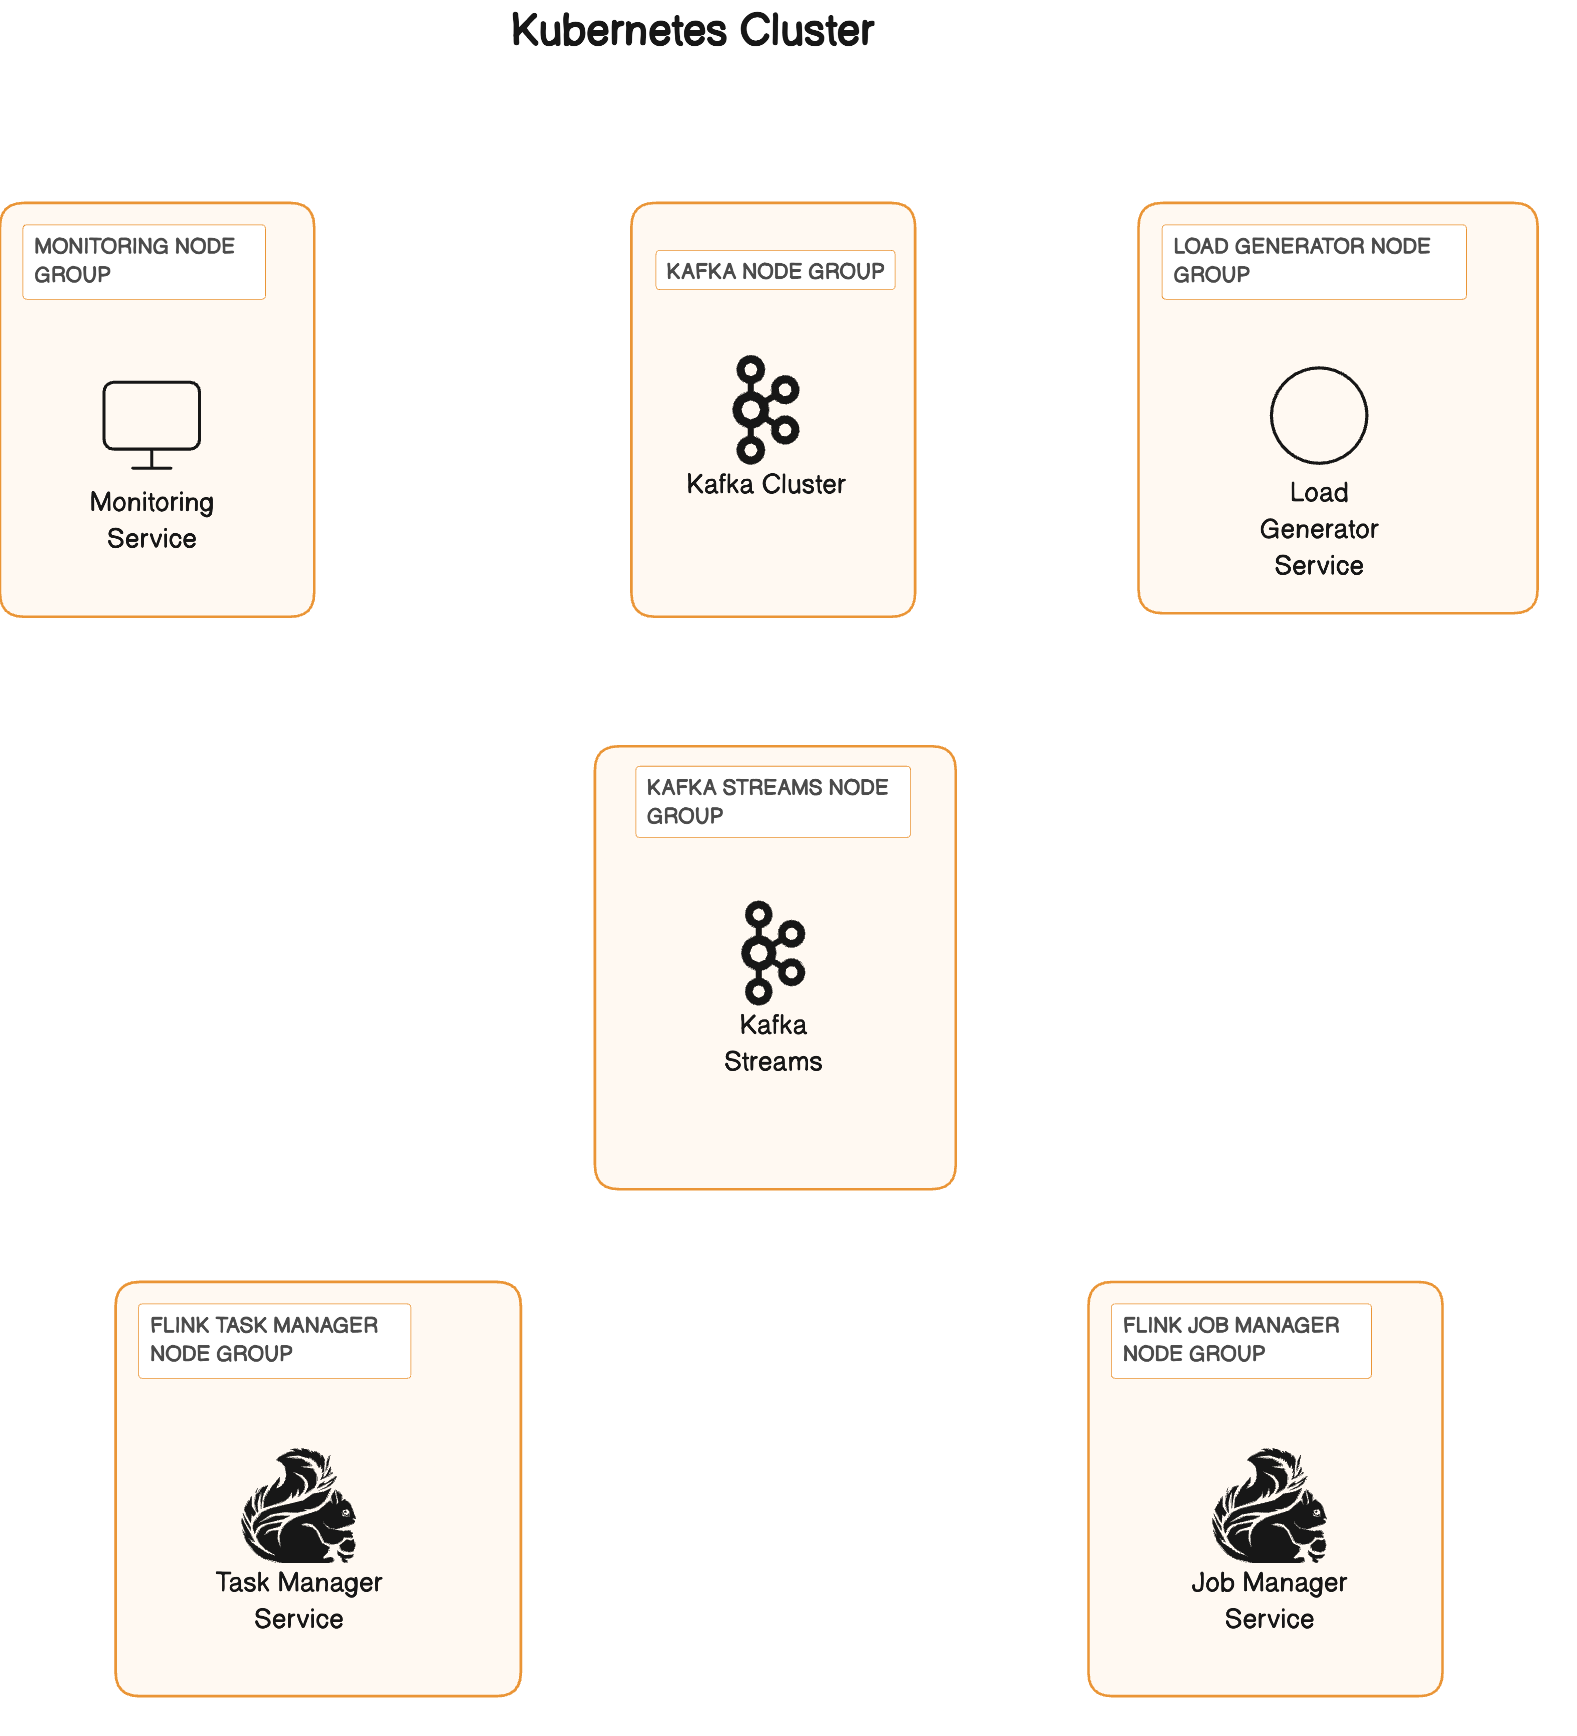
\includegraphics[width=1\textwidth]{figures/eks-node-groups}
    \caption{\textit{Node groups for the case study experiments.}}
    \label{fig:node-gorups}
\end{figure}


\newpage
\section{Kubernetes cluster setup}\label{subsec:eks-cluster-configuration}
This section is describing Kubernetes cluster and key components which are running
with during experiments execution to collect metrics.

\subsection{EKS node groups}\label{node-groups}

As shown on Figure \ref{fig:node-gorups}, the setup is based on 5 node groups, with the following
node types \cite{aws_node_types}.

\begin{description}
    \item[Kafka node gorup] 3 Kafka brokers, where each broker gets deployed to a separate node.
    Such that several brokers never run on the same node.
    Node types for this group is m6i.2xlarge \cite{aws_node_types}.
    \item[Load generator node group] Is Java based application which generates Kafka messages of 1Kb size
    to Kafka input topic with 50 partitions.
    In this study two load generator instances are used where each generates 100000 messages per second.
    Node types for this group is m6i.xlarge.
    \item[Manager node group] The following node groups is intended only for Apache Flink task manager \cite{flinkArchitecture2024} instance of 1 replica
    and is not used for experiments with Kafka Streams.
    \item[Infra node group] This node group is used for benchmarking tools deployment such as EBS, EFS controllers,
    Grafana, Theodolite operator, Prometheus, Chaos Mesh and additional operators which are used only for data collection
    and visualisations.
    Should not affect workers and load generators.
    Node types for this group is m6i.xlarge.
    \item[Worker node group] This node group is used for Kafka Streams setup and Apache Flink task managers \cite{flinkArchitecture2024}.
    Such that stream processing replicas are running on a separate nodes, where each node has only one worker replica
    running in the node.
    Detailed worked groups is shown on Figure \ref{fig:worker-node-group}.
    For this case study were chosen 8 nodes with 8 workers replicas.
    Node types for this group is c5.large.
\end{description}


\begin{figure}[ht]
    \centering
    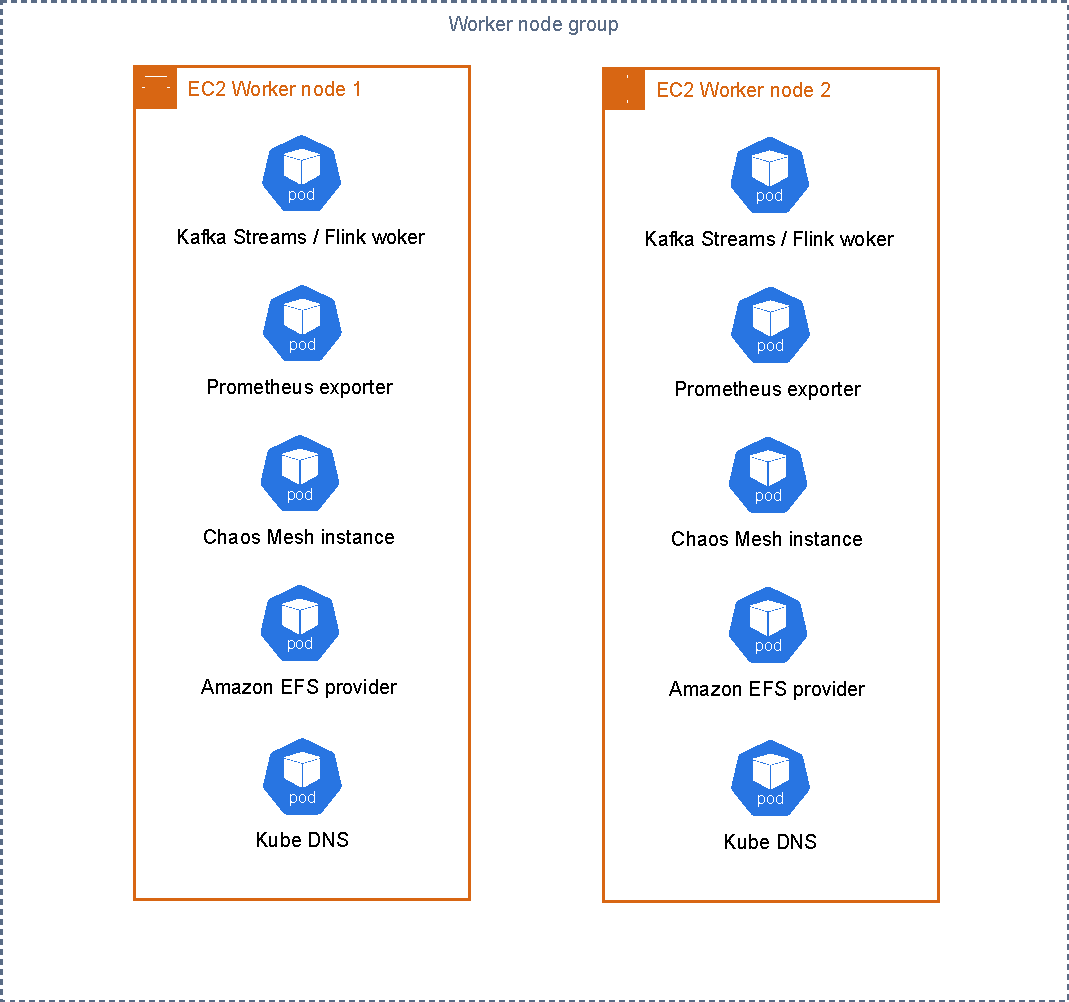
\includegraphics[width=1\textwidth]{figures/worker-node-group}
    \caption{\textit{Worker node group with 2 nodes and pods in each node.}}
    \label{fig:worker-node-group}
\end{figure}


\subsection{EFS and EBS storage services}\label{storage-services}

\begin{figure}[ht]
    \centering
    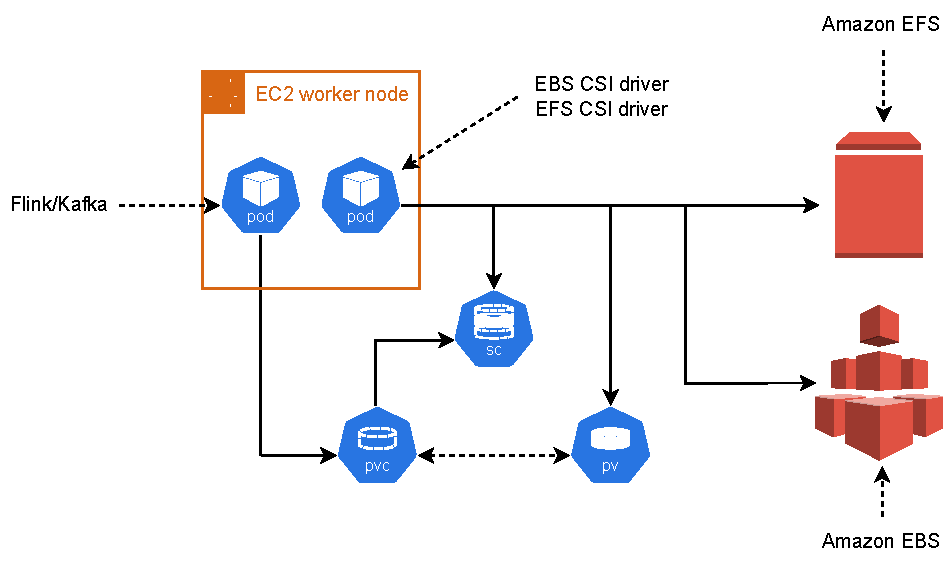
\includegraphics[width=1\textwidth]{figures/aws-storage-pvc}
    \caption{\textit{EBS and EFS network storage diagram.}}
    \label{fig:aws-storage}
\end{figure}

Stream processing uce case is data intensive in this study.
To be able to handle data loads during experiments were chosen two storage services
for storing the data.
These storage are EFS \cite{awsEFS}, and EBS \cite{awsEBS}.
AWS provides networks storage types for EC2 nodes \cite{EC2} which are used
for storing a big amount of data.
The crucial part of this network storage is that if worker on node goes down for some time,
then saved state won't be lost.
A real physical node is connected to the network storage via a network configuration as it shown on Figure \ref{fig:aws-storage}
which is also described in details in the following documentation \cite{awsKubernetesStorage}.
Such a complex model gives pod a network connection to a physical storage such that huge amount
of data gets written and read fast enough for production systems.
The diagram on Figure \ref{fig:aws-storage} includes several the following components.

\begin{description}
    \item[Flink and Kafka pods] These are Java application which use networks storage.
    For thi study Flink workers use EFS storage for storing stages and Kafka brokers
    use EBS for Kafka topics.
    \item[EBS and EFS CSI drivers] Cloud tool provided by AWS to manage network connection
    between nodes and networks storage.
    Driver runs on the same node as Kafka brokers and Flink worker to get network storage access.
    \item[PV] Persistent volume gives networks access to a physical storage, where the state gets saved.
    \item[PVC] Persistent volume claim is Kubernetes abstraction that connects to PV.
\end{description}


\section{Metrics exporters}\label{sec:metrics-exporters}
This section cover how a Theodolite framework \cite{theodolite_framework} is used
to get metrics and to run experiments in cloud environment.

\subsection{Kafka metrics exporters}\label{subsec:metrics-exporters}
Theodolite comes with a set of tools which are used to export metrics from running pods.

\begin{figure}[ht]
    \centering
    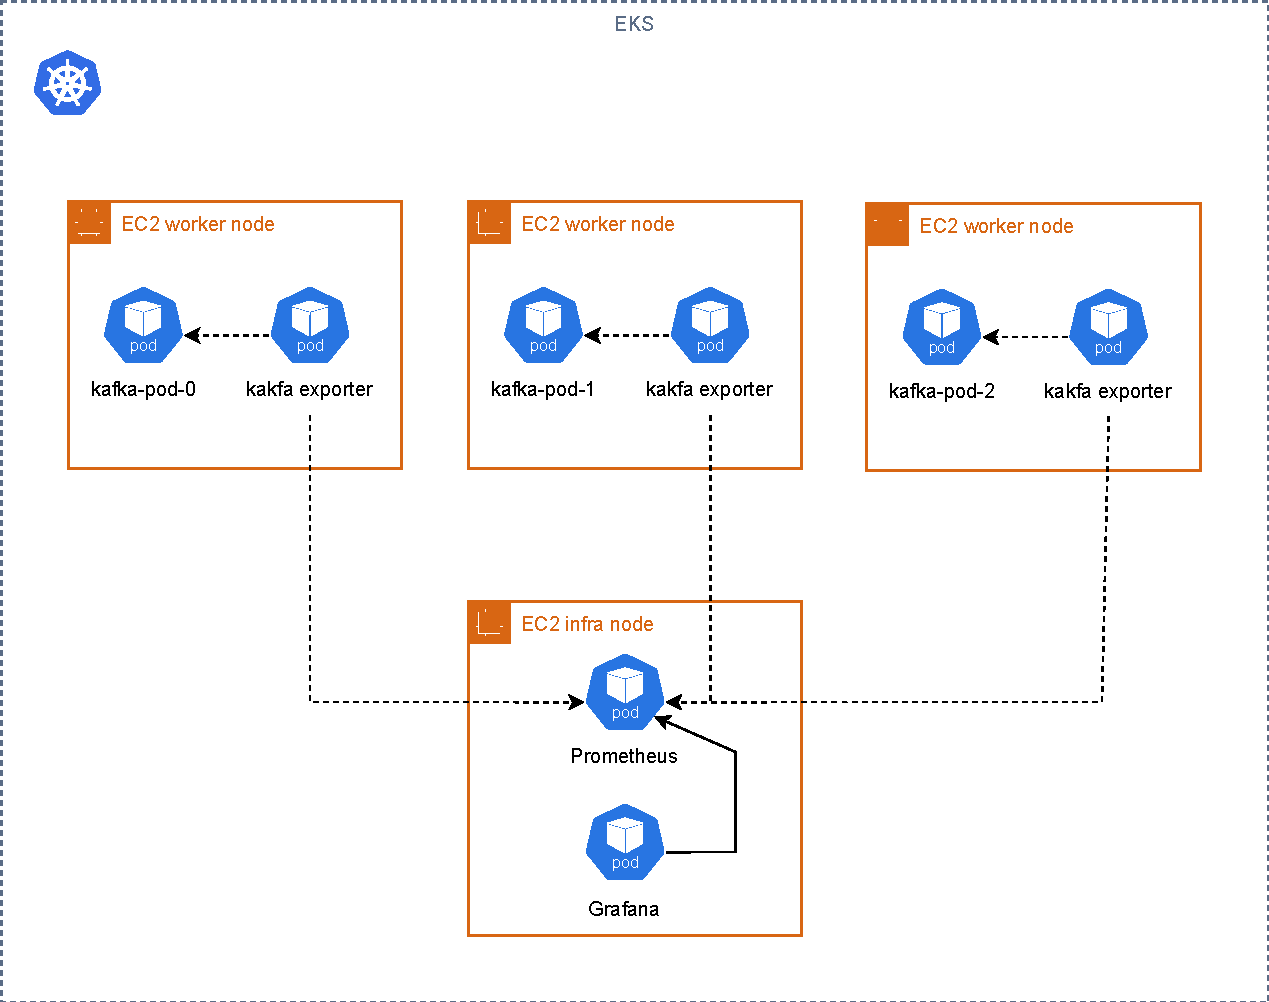
\includegraphics[width=1\textwidth]{figures/kafka-exporter}
    \caption{\textit{Kafka metrics exporter that sends metrics from JMX exporter to Prometheus.}}
    \label{fig:kafka-exporter}
\end{figure}

On Figure \ref{fig:kafka-exporter} is an example of Kafka metrics exporter.
It reads metrics from Kafka's JMX exporter about consumer groups, commit lag, topics,
topic partitions, topic offsets.

\newpage
\subsection{Kubernetes and worker metrics exporters}
Kubernetes setup in this study is coming with Kubernetes metrics services \cite{kubernetesResourceMetrics} which are
configured by Theodolite.
Metrics diagram is depicted on Figure \ref{fig:metrics-collection}.

\begin{figure}[ht]
    \centering
    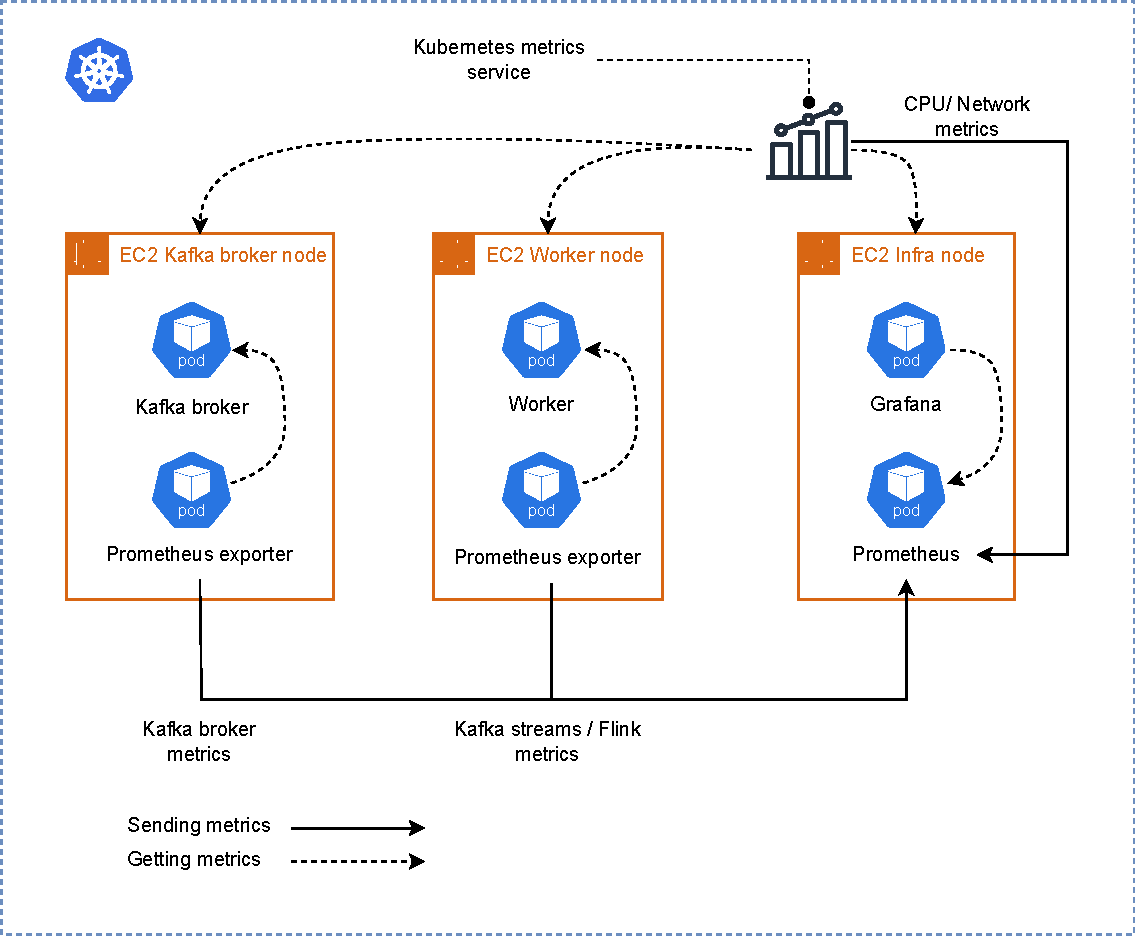
\includegraphics[width=1\textwidth]{figures/metrics-collection}
    \caption{\textit{Kubernetes and worker metrics exporters.}}
    \label{fig:metrics-collection}
\end{figure}

Kubernetes metrics services expose metrics about node network utilization and CPU consumption.
All exposed metrics get saved to Prometheus that makes them accessible by executing PromQL.
For example, Grafana queries PromQL queries to plot real time charts with used cluster resources.

\subsection{Latency exporter}\label{subsec:latency-exporter}
The Latency exporter measures the latency between when a message was generated by load generator and when
it was committed to a Kafka log.
Provides positive and negative latencies as metrics that are available in Prometheus as p50, p90, p95.
These latencies get calculated by micrometer \cite{micrometer}.

\begin{description}
    \item[Positive Latency] If the latency is positive (a message commit time is later than event time).
    \item[Negative Latency] If the latency is negative (a message commit time is earlier than event time)
\end{description}


\section{Benchmarks setup}\label{sec:benchamrks-setup}
Theodolite is responsible for a full lifecycle of benchmarks execution with
a set of Kubernetes deployment configurations.
The General diagram is depicted on Figure \ref{fig:theodolite-process}.

\begin{figure}[ht]
    \centering
    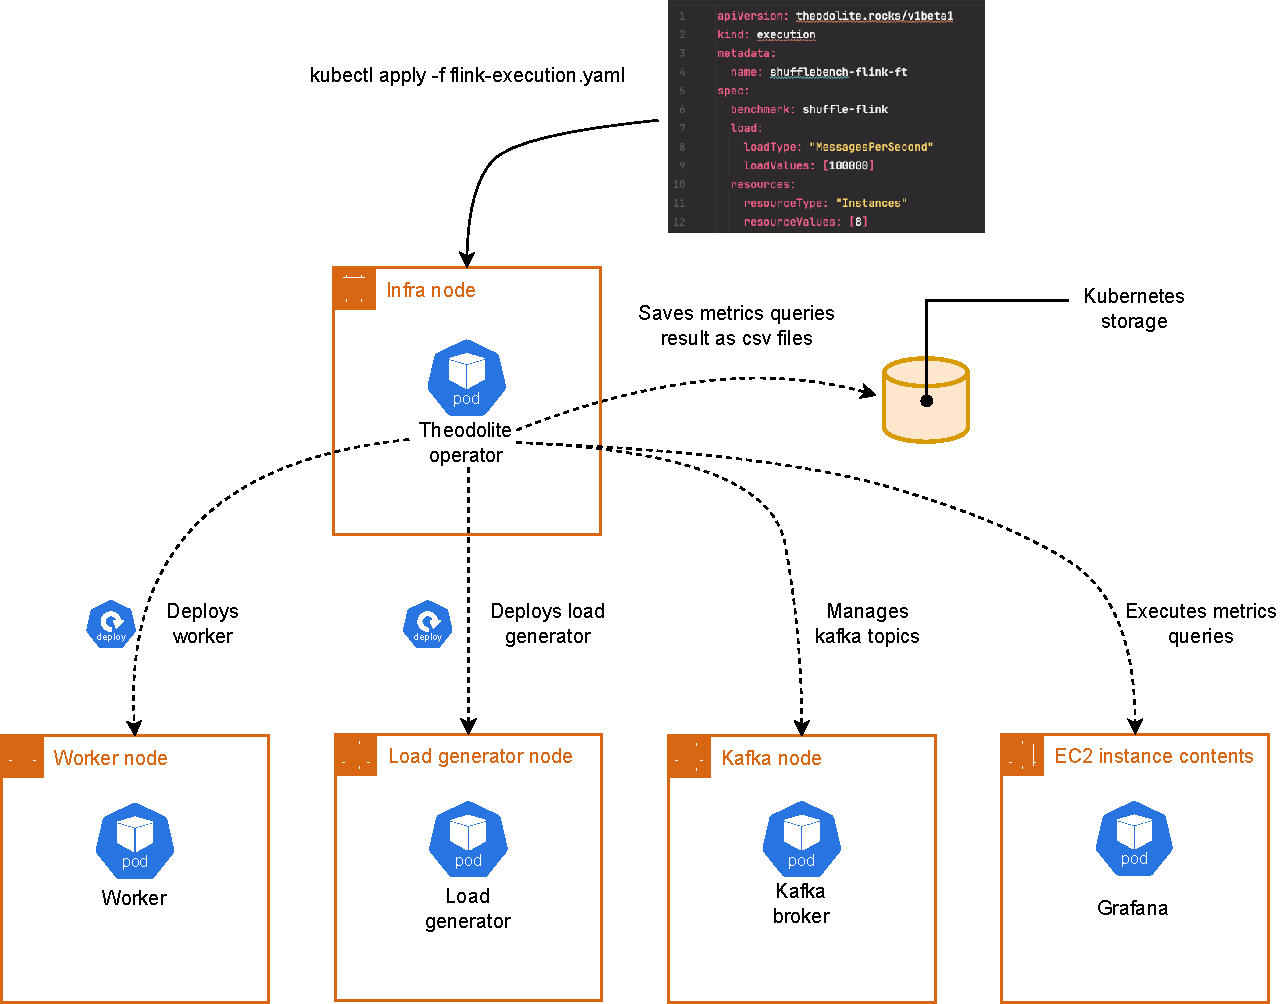
\includegraphics[width=1\textwidth]{figures/theodolite-process}
    \caption{\textit{Theodolite manages deployment and undeployment of load generator and workers during experiment execution.}}
    \label{fig:theodolite-process}
\end{figure}

To run execution with Theodolite, some preconfiguration has to be made.
Theodolite needs to get access to Kubernetes deployment files for Kafka Streams,
Apache Flink.
Deployment for load generator and monitoring tools comes with Theodolite our of the box.
For custom usage, it is possible to override some deployment configurations.
Apache Flink and Kafka Streams deployment files have to be stored in Kubernetes as config maps \cite{kubernetesConfigMap}.
After each benchmark execution, Theodolite automatically undeploys load generator and workers.


\section{Chaos engineering with Chaos Mesh}\label{sec:chaos-mesh}

\begin{figure}[ht]
    \centering
    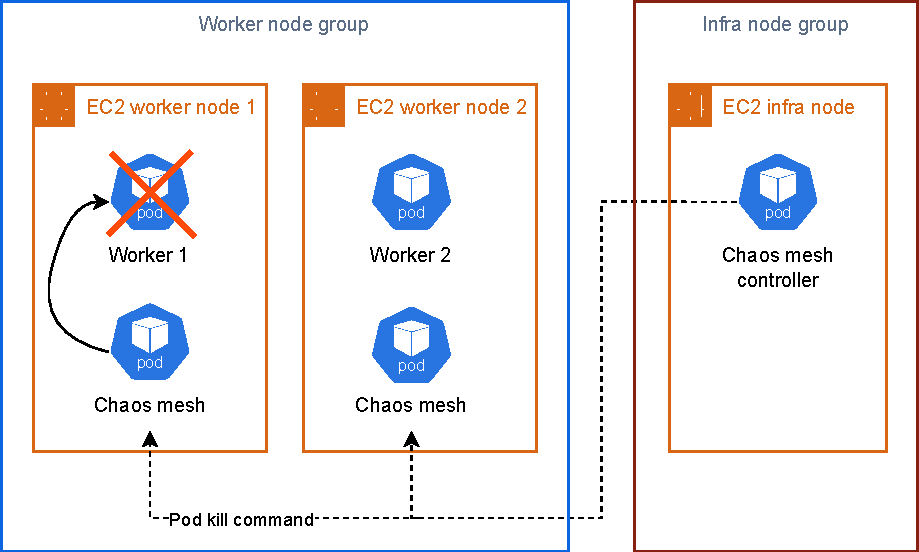
\includegraphics[width=1\textwidth]{figures/mesh-pod-kill}
    \caption{\textit{Example of Chaps Mesh periodic Pod kill. Chaos Mesh controller selects Chas Mesh daemon to
    and sends a message to kill the worker.}}
    \label{fig:chaos-mesh-kill}
\end{figure}

Chaos Mesh \cite{chaosMesh} is a tool used in the Kubernetes environment to simulate
different kinds of failures.
In this case study it is used to kill worker node by using pod selector.
Each deployed worked has its own label, for example, type:worker.
For all experiments, Chaos Mesh is configured to kill worker pods every 3 minutes.
An example use of Chaos Mesh in this case study is depicted on Figure \ref{fig:chaos-mesh-kill}.
Chaos Mesh installs Chaos daemon on each worker node, such that has
Chas Mesh contoller has access to worker pods for failure simulation.
However, Kubernetes quite fast redeploys killed worker replicas, but this time is more than enough
to find valuable metrics about how the system would behave.
For example, Kafka Streams and Apache Flink use different re-partitions algorithms to
handle load balancing.
Depending on re-partitions strategies, this case study can show this difference by measurement
a stare recovery time.

\section{Experiment setup}\label{sec:experiment-setup}
This section describing experiment execution steps to show how to deploy benchmarks setup and
get benchmarks as csv files from scratch.

\subsection{Prerequisite}\label{subsec:prerequisite}
To get started with benchmarks execution, some steps need to be finished first.

\begin{description}
    \item[Prototype compilation] Build prototypes source code.
    \item[Docker images] Once code is compiled, Docker images need to be built and deployed
    to ECR \cite{awsECR} service which is AWS image storage.
    \item[Kubernetes Deployment configuration] Configure deployment configuration files for Apache Flink
    and Kafka Streams prototypes.
\end{description}

Built Docker images and configured Kubernetes deployment files are
prerequisite to get started with Theodolite and EKS deployment.

\subsection{EKS cluster}\label{subsec:eks-cluster}
Execute command with eksctl tool EKS cluster configuration in cluster.yaml  \ref{lst:eks-cluster}.

\begin{lstlisting}[label={lst:eks-cluster}]
    eksctl create cluster -f cluster.yaml
\end{lstlisting}

Once the cluster is created, EBS and EFS network storage have to be configured.
For EFS the following installation guide needs to be done first \cite{awsEfsCsi}.
The Next step is applying EBS and EFS storage configuration \ref{lst:eks-storage}.

\begin{lstlisting}[label={lst:eks-storage}]
    kubectl apply -f kafka-storage-class.yaml
    kubectl apply -f flink-storage-class.yaml
\end{lstlisting}


\subsection{Theodolite configuration}\label{subsec:theodolite-isntllation}
Prerequisite is values.yaml with defined node selector for EKS node groups,
it should not be installed to worker and load generator nodes.

\begin{lstlisting}[label={lst:theodolite-inst}]
    helm install theodolite theodolite/theodolite -f values.yaml
\end{lstlisting}

These Kubernetes config maps load deployment files to Kubernetes config such that Theodolite
has access to files within Kubernetes.
\begin{lstlisting}[label={lst:config-map}]
    kubectl create configmap --from-file ./shuffle-load-generator/
    kubectl create configmap --from-file ./shuffle-latency-exporter/
    kubectl create configmap --from-file ./shuffle-kstreams/
    kubectl create configmap --from-file ./shuffle-flink/
\end{lstlisting}


These commands tell Theodolite how to access config maps created in a previous step \ref{lst:config-map}.
\begin{lstlisting}[label={lst:config-map-theodo}]
    kubectl apply -f theodolite-benchmark-kstreams.yaml
    kubectl apply -f theodolite-benchmark-flink.yaml
\end{lstlisting}

At this step, deployment configurations should be ready to be used during experiments.


\subsection{Running experiments}\label{subsec:running-experiments}
To run experiments, Thedolite is listening for execution files to be applied but
kubectl.
Theodolite Kubernetes execution file represents instruction for Theodolite operator
about how to run experiments.
For example, what services to deploy, how log should experiment be running, environmental
variables, how many repeats have to be.
Experiment execution could be described in the following steps:

\begin{description}
    \item[Appy execution config] Once Theodolite operator found the execution config, it's
    starting deploying components which are need to be running only during the experiment execution.
    In this case study, these are: load generator, latency exporter, Kafka Streams or Apache Flink
    workers replicas.
    \item[Running experiment] Based on the execution config, the experiment is running for a certain
    time period, in this case study it's 18 minutes.
    \item[Finishing experiment] Once the execution time has passed, Theodolite operator undeploy,
    deployed services at execution start, executes PromQL queries to get benchmarks from Grafana,
    and saves them as CSV files.
\end{description}

Examples of csv files are shown in

\begin{lstlisting}[label={lst:bench-csv-files}]
    exp3_managerNodesDiskReadMB_2s_1.csv
    exp3_generic_latency_p90_30s_1.csv
    exp3_kafkaBrokerNodesCPUsPercentageUtilization_2s_1.csv
    exp3_workerNodesCPUsPercentageUtilization_2s_1.csv
\end{lstlisting}


%\section{Benchmarks metrics}\label{sec:benchmarks-metrics}
%Benchmarks setup for the case study is exploring the following metrics:
%
%\begin{itemize}
%    \item Average worker nodes CPU utilization.
%    \item Output throughput per broker.
%    \item Output throughput per partition.
%    \item Input throughput per broker.
%    \item Input throughput per partition.
%    \item Input throughput.
%    \item Kafka broker node CPU utilization.
%    \item Kafka broker nodes disc read.
%    \item Kafka broker nodes disc write.
%    \item Kafka broker nodes network received.
%    \item Kafka broker node networks transmitted.
%    \item Kafka input topic lag per partition.
%    \item Kafka laf per repartition.
%    \item Kafka message latency p50.
%    \item Kafka message latency p90.
%    \item Kafka message latency p95.
%    \item Kafka message latency p99.
%    \item All nodes CPU utilization.
%    \item Number of worker replicas.
%    \item Output throughput.
%    \item Pods CPU percentage utilization.
%    \item Pods CPU total utilization.
%    \item Pods IO memory ped pod.
%    \item Pods network received.
%    \item Pods network transmit.
%    \item Worker nodes CPU utilization.
%    \item Worker nodes disk read.
%    \item Worker nodes disk write.
%    \item Worked nodes network received.
%    \item Worker nodes network transmit.
%    \item Kafka consumer group lag trend.
%\end{itemize}
%
%Based on the metrics above, the case study is trying to make a
%conclusion about performance difference between Kafka Streams and Apache Flink
%in case of fault tolerance with a state recovery.

%\subsubsection{Load Generator}
%The load generator is only designed to generate a stream of Kafka messages, where
%each message is a random byte array of 1KB size.
%The generator is based on a simple spring boot app, where the load of messages is
%generated with ScheduledThreadPoolExecutor of 4 threads.
%A nature of the mode generator requires more cpus rather than a disc space.
%
%The node group of the generator consists only of a single node of a type m6i.xlarge.
%This node is efficient enough to generate 200K MPS and even much more.
%
%\subsubsection{Kafka Streams}
%Kafka Streams as well as the load generator is based on Spring Boot framework since it is
%the mose popular and common framework for running Java applications and provides out of the box
%support for Kafka Streams.
%It's important to have as fewer configurations as possible to simply run and Deploy Kafka Steams
%instance.
%Kafka Steams node groups consists of m6in.xlarge type nodes.
%
%\subsubsection{Apache Flink}
%Apache Flink requires a different approach for node groups comparing to Kafka Streams since
%it has a different architecture and includes additional components to run and manage streaming
%jobs.
%For this benchmarking experiments two separate node groups were used.
%The first one of for Flink job manager and the second one is for Flink task managers which
%are workers.
%Flink job managers require much less resources since they are intended to control task managers.
%For these experiments for task managers was chosen a node groups of type t3.medium.
%For task managers was chosen a more performant node type m6in.xlarge.
%The same type was used for Kafka Streams to compare a resource consumption for two solutions.
%
%However, these experiments required additional component for the Flink cluster which is
%Flink Kubernetes Operator.
%It is open source and open source solution to dramatically simplify a Flink cluster management.
%For experiments, it was running withing the monitoring node group since it doesn't consume
%many resources.
%
%\subsubsection{Monitoring}
%The following group was used as a default node group for any other services, like Prometheus,
%Grafana, Prometheus Operator, Flink Operator.
%Monitor node groups consists of two nodes of type t3.medium.
%
%\subsection{Infrastructure as Code}\label{subsec:infrastructure-as-code}
%With such complex cloud setup, it's simple not possible to create and such
%complex infrastructure and fortunately there are available tools for such use cases.
%The main tools which were used for experiments are \textbf{Helm} and \textbf{kubectl}
%
%\begin{description}
%    \item[Helm] is a tool which manages packages for Kubernetes cluster, it allows to create,
%    update and deleted Kubernetes resources.
%    \item[kubectl] is a cli tools which also allows to manage resources, but not as a package but
%    rather each resource separately.
%\end{description}
%
%For experiments, were create all required Kubernetes resources which makes deployment
%quite fast and efficient.
%
%For each experiment there's a set of Kubernetes resource files which is used
%for a specific benchmark.
%It makes deployment easier and less error-prone, however it might bring
%too much boilerplate code.



%\section{Implementation Details}\label{sec:implementation-details}
%This section covers use case implementation with Kafka Streams and Apache Flink.
%The source code for Apache Flink and Kafka Streams is Java Gradle based project,
%where gradle version is 8.5 and jar were build with Java 11 and Java 21.
%Both builds were deployed to Amazon ECR, such that once deployed Docker images
%are reusable and not required to be built for each experiment separately.
%The core image built platform is Docker.
%In order to deploy build images two cli tools were used.
%
%\begin{description}
%    \item[Docker cli] is a tool which help to build Docker images with the app and deploy them
%    to Kubernetes cluster.
%    Quite important to use a correct platform, for experiment were chosen Linux distros, for
%    this reason the following build parameter was used --platform=linux/amd64.
%    Moreover, docker cli provide aws login system which knows how to deploy build images directly to
%    Amazon ECR.
%    \item[aws cli] is a cli which provides API to work with AWS resources, docker cli
%    is integrated with the aws cli quite well.
%\end{description}


%\subsection{Rule Based Matcher}\label{subsec:rule-matcher}
%
%\begin{figure}[H]
%    \centering
%    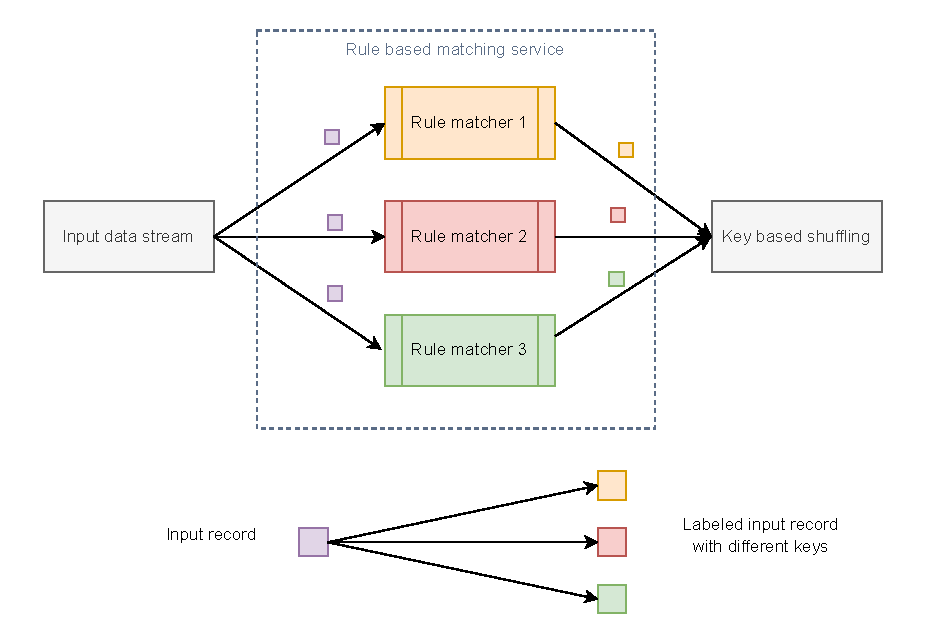
\includegraphics[width=1\textwidth]{figures/rule-matcher}
%    \caption{\textit{Rule based matcher.}}
%    \label{fig:rule-matcher}
%\end{figure}
%
%This is the core component of streaming pipeline for the use case.
%It could be considered as a black box which provides a single api method to match
%incoming bytearray record.
%Its logic could be described using diagram above ~\ref{fig:rule-matcher}.
%
%The matched has a single method interface for byte array record which
%can based on defined rules is able to matched with them.
%All matched rules get shuffled by name which makes to distributed
%further processing among all replicas.
%The main parameters of the matcher are selectivity and number of rules.
%
%\begin{description}
%    \item[Matching Rule] is a rule which has a selectivity property to be matched with a byte array record.
%    \item[Selectivity] is a value with a floating point which defined a probability witch record can be
%    matched.
%\end{description}
%
%For example, if the matcher has 10000 rules, with selectivity of 0.00002, then a probability with
%which it will be matched with incoming record is 0.00002\%.
%These values could be different depending on a system simulation.
%The matcher is a prototype which is supposed to simulate a real service.
%Since the rule matched is not a focus of the research, it is more than enough to use
%a prototype.

%\subsection{Kafka Streams Implementation}\label{subsec:kafka-streams-implementation}
%
%\begin{figure}[H]
%    \centering
%    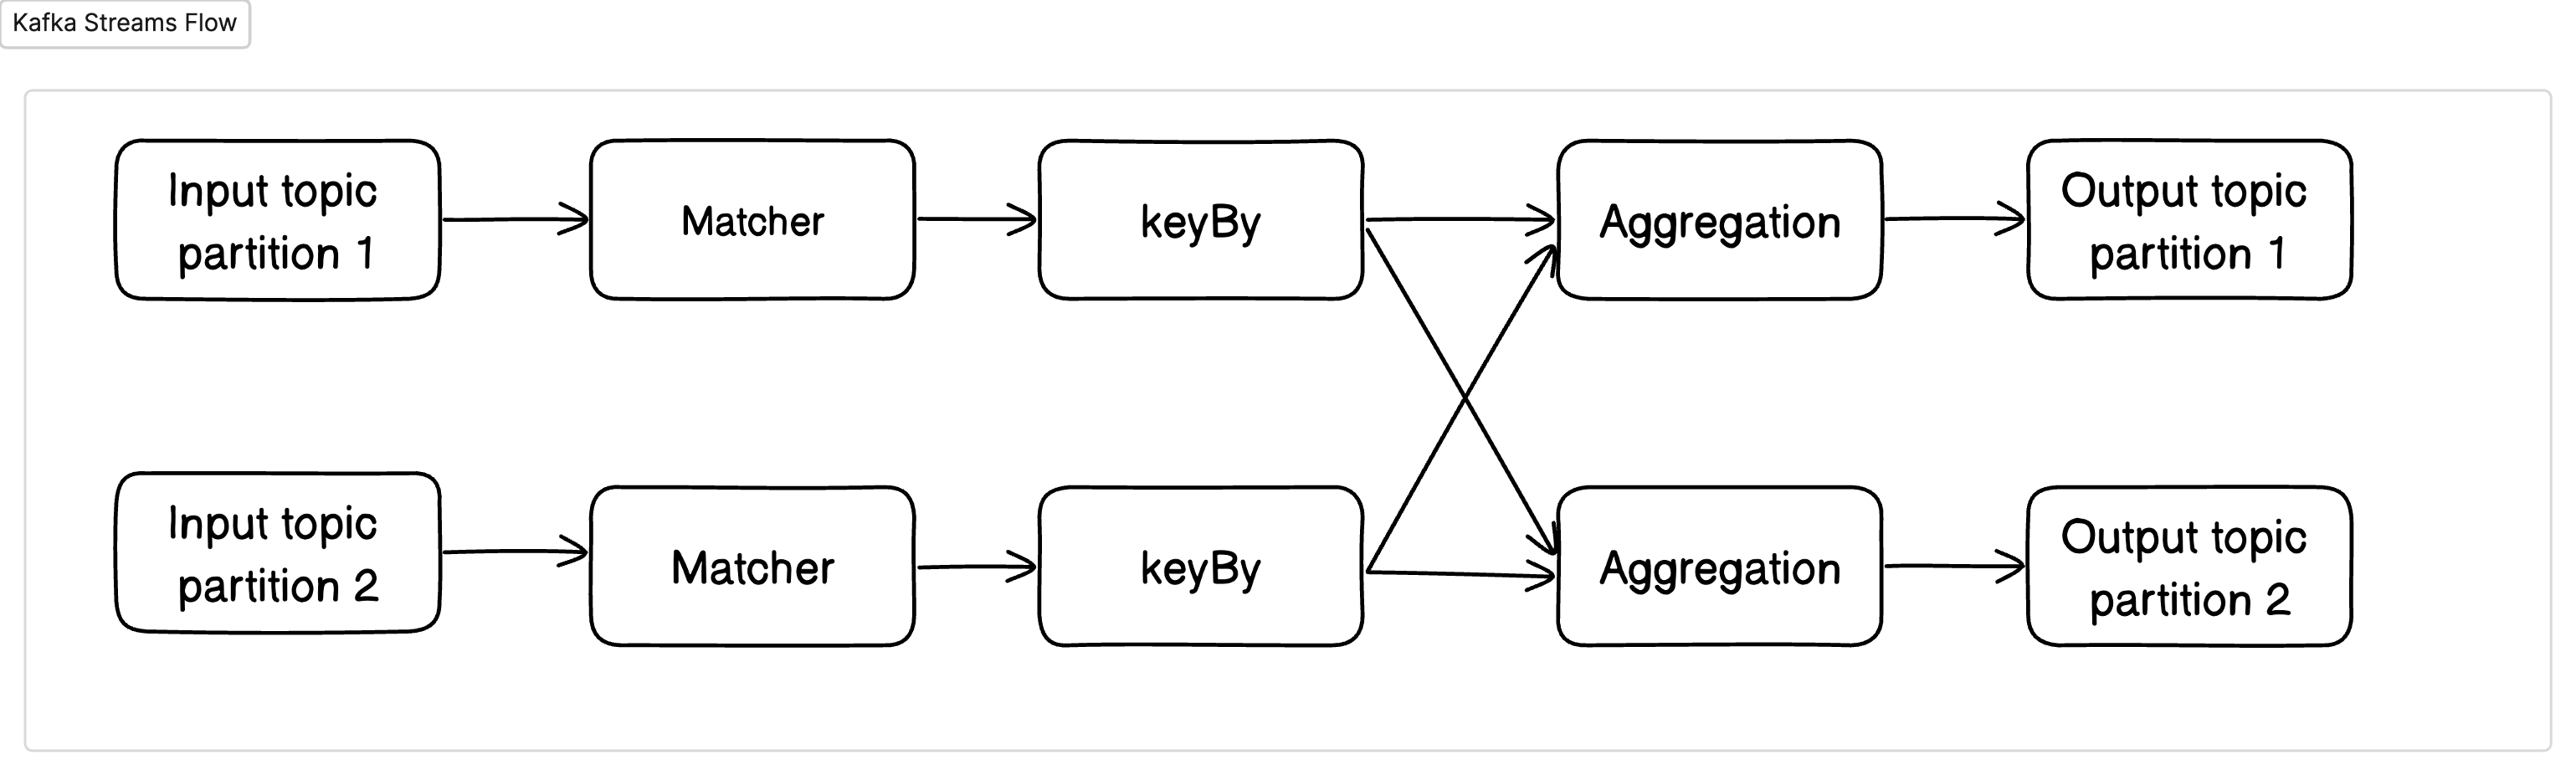
\includegraphics[width=1\textwidth]{figures/k-streams-shuffle}
%    \caption{\textit{Kafka Streams flow.}}
%    \label{fig:k-stream-shufle}
%\end{figure}
%
%Kafka Streams flow is presented on the figure above ~\ref{fig:k-stream-shufle}.
%For the experiments Kafka Streams use default configurations with Kafka
%commit time period of 30 seconds.
%
%
%\subsection{Flink Implementation}\label{subsec:flink-implementation}
%
%\begin{figure}[H]
%    \centering
%    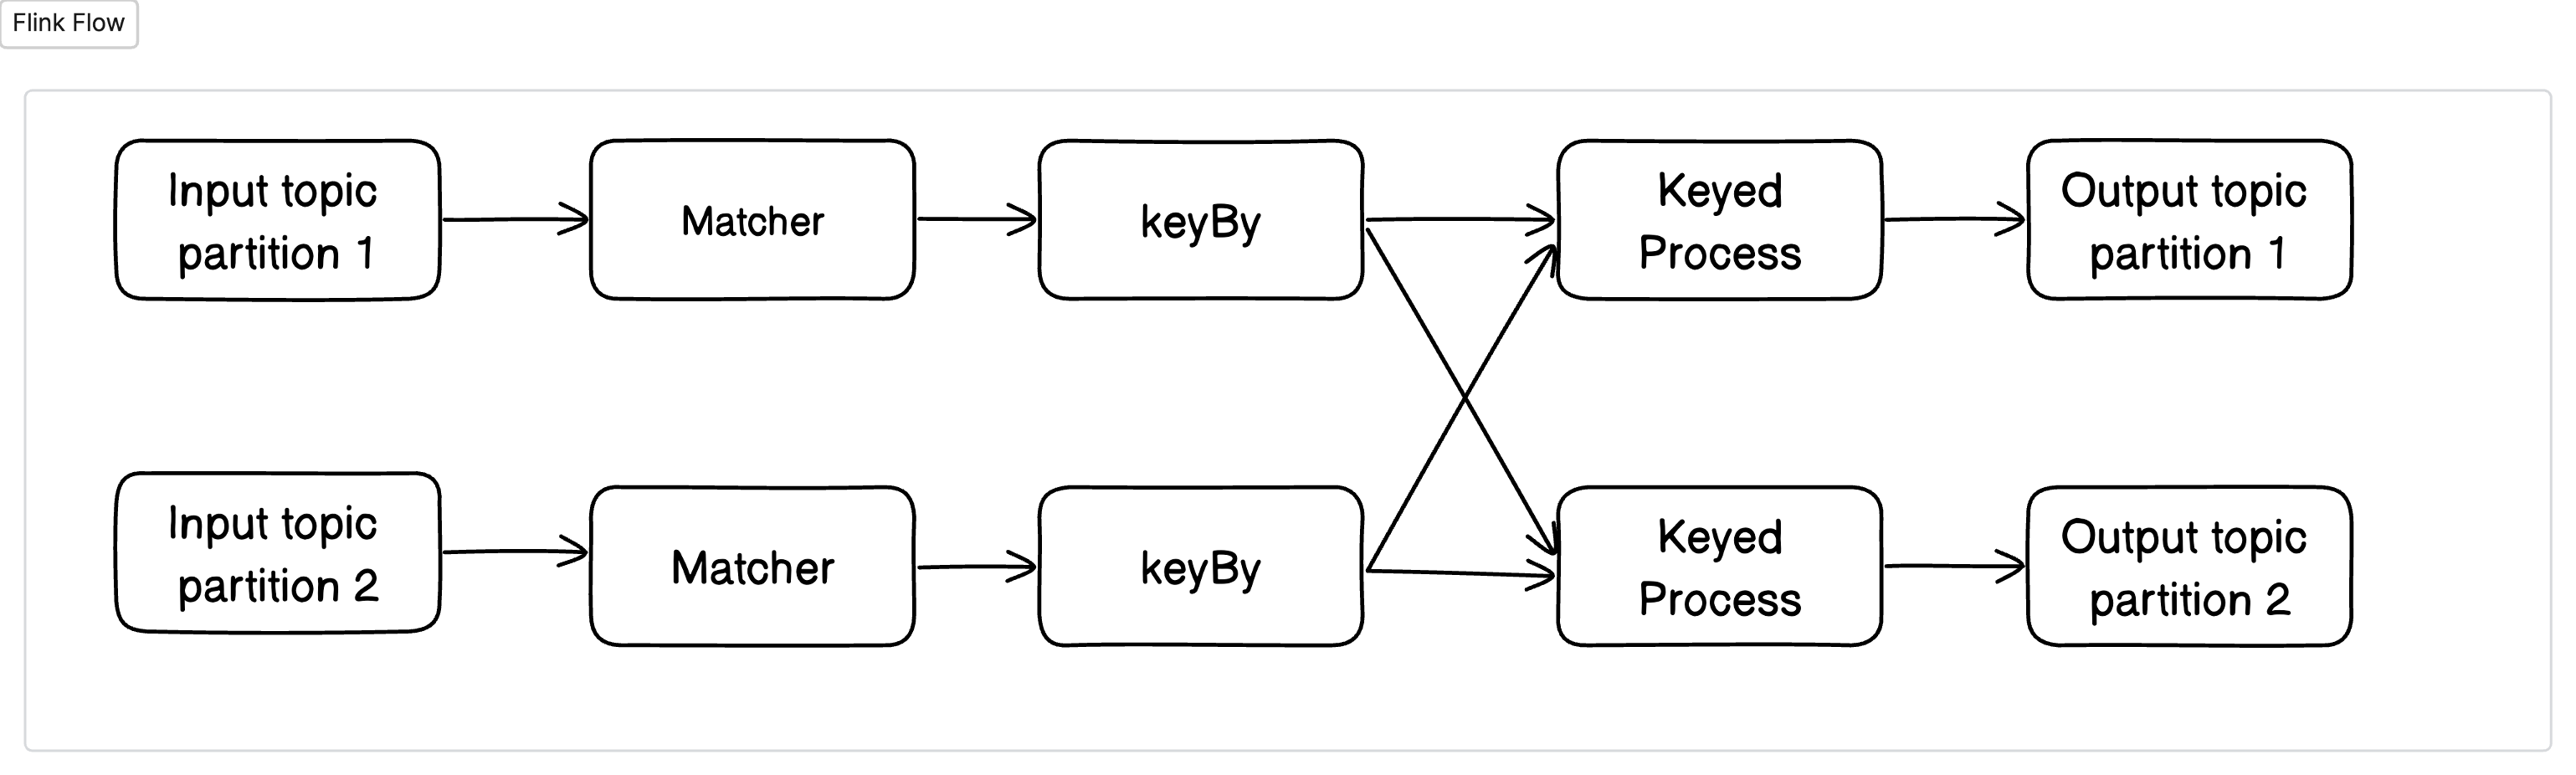
\includegraphics[width=1\textwidth]{figures/flink-shuffle}
%    \caption{\textit{Flink flow.}}
%    \label{fig:flink-shuffle}
%\end{figure}
%
%Flink is using keyed process which also type of aggregation but with a little
%bi different behaviour.
%Flink implementation uses checkpoints, which are get saved every 30 seconds
%to Amazon S3 storage.
%It was done to get the Kafka commit interval like in
%Kafka Streams implementation.
%The same commit interval helps to compare a performance difference.
%
%However, experiments with Flink require to install to EKS cluster additional
%dependencies which are need to manager Flink cluster.
%These tools are: cert-manager for Kubernetes cluster, Flink Kubernetes Operator,
%RBAC roles and permission for Flink Operator which must be allowed to
%deploy Flink task managers and job managers.
%
%

